\documentclass[t, 				             
			   final, 				         
			   xcolor={usenames,dvipsnames}, 
			   table]{beamer}

% pacotes utilizados.
\usepackage{amsmath}
\usepackage[brazil]{babel}
\usepackage[utf8]{inputenc}
\usepackage{booktabs}
\usepackage[alf]{abntex2cite}
\usepackage{caption}


\usepackage{todo}

% configuração do tema
\usetheme[pageofpages=de,
          bullet=square,			
          titleline=true,				
          alternativetitlepage=true,			
          titlepagelogo=imagens/logo-unicamp,	
          watermarkheight=70px,		
          watermarkheightmult=4	
          ]{Torino}

\setbeamertemplate{sections/subsections in toc}[square]
\setbeamertemplate{bibliography item}[default]

\usecolortheme{freewilly}

\logo{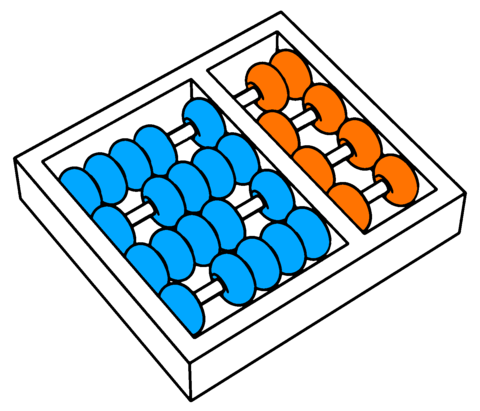
\includegraphics[height=0.110\paperheight]{imagens/logo-ic}}

\begin{document}
    \author{Luiz Alberto Ferreira Gomes}
\title{Manutenibilidade em Linhas de Produtos de Software}
\subtitle{Projeto de Interface de Usuário  }
\institute{Instituto de Computação}
\date{\today}

    \begin{frame}[plain]
  \titlepage
\end{frame}
    \AtBeginSection[]
{
  \begin{frame}{Agenda}
    \tableofcontents[currentsection]
  \end{frame}
}
  
    \section{Conceituação Básica}

\begin{frame}[t, fragile]{Manutenção de Software}
    \begin{block}{Definição:}
    \alert{Modificação} do produto de software \alert{após} a sua colocação em \alert{uso} \textcolor{Blue}{\cite{Sommerville2011}}.
    \end{block}
    
    \begin{figure}[hbt]
    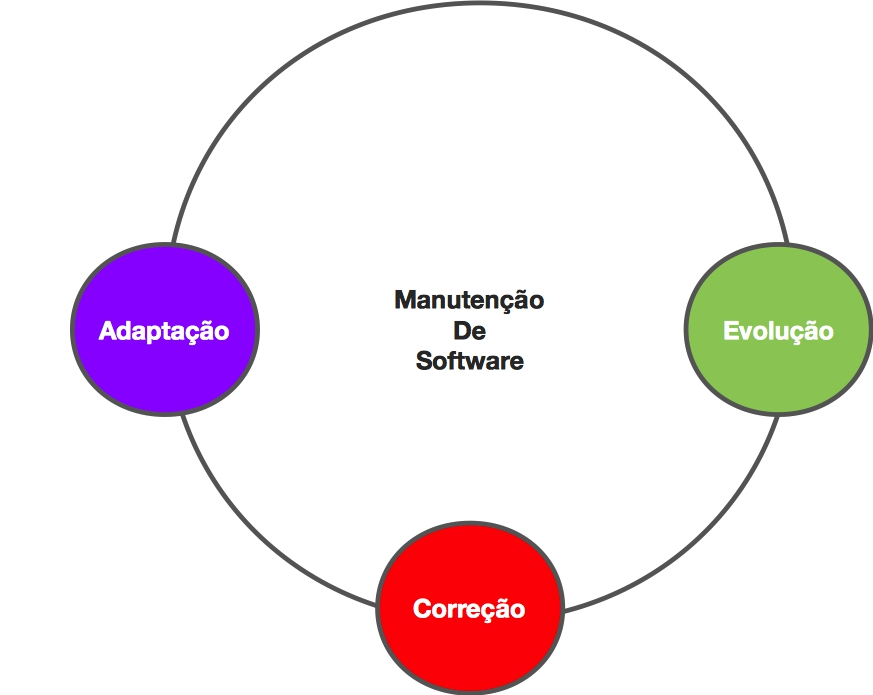
\includegraphics[width=0.5\textwidth]{imagens/tipos-de-manuntencao.jpg}
  \end{figure}
    
\end{frame}

\begin{frame}[t, fragile]{Manutenibilidade}
    \begin{itemize}
      \item \alert{Não} existe um \alert{entendimento} comum sobre o que é \alert{manutenibilidade}, como
        ela pode ser \underline{atingida}, \underline{medida} e \underline{avaliada}
%      \begin{itemize}
%        \item Diferentemente de outros atributos como desempenho
%        \item Toda organização de software de tamanho significativo parece ter a sua própria definição
%        de tamanho
%      \end{itemize}

%      \item O glossário de termos da IEEE define \alert{manutenibilidade} assim:
%      \begin{itemize}
%        \item \textbf{Manutenibilidade} mede a \alert{facilidade} com que o sistema pode ser \alert{modificado} para corrigir falhas, 
%        melhorar o desempenho ou outros atributos, ou adaptar à mudanças no ambiente \textcolor{Blue}{(IEEE)}.
%%      \end{itemize}
%%\framebreak       
%%      \item O Software Engineering Institute define \alert{manutenibilidade} assim:
%%      \begin{itemize}
%        \item \textbf{Manutenibilidade}  \alert{esforço} necessário para realizar \alert{modificações} na \alert{implementação} de um componente específico \textcolor{Blue}{(SEI)}.
%      \end{itemize}
%\framebreak      
%      \item A norma ISO/IEC 9126 define \alert{manuteniblidade} assim:
      %\begin{itemize}
      
  \end{itemize}
  \begin{block}{Definição:}
        \textbf{Manutenibilidade} mede o \alert{esforço} necessário para fazer \alert{modificações} específicas no software \textcolor{Blue}{\cite{Cortes2001}}.
      \end{block}
  
  \begin{figure}[hbt]
    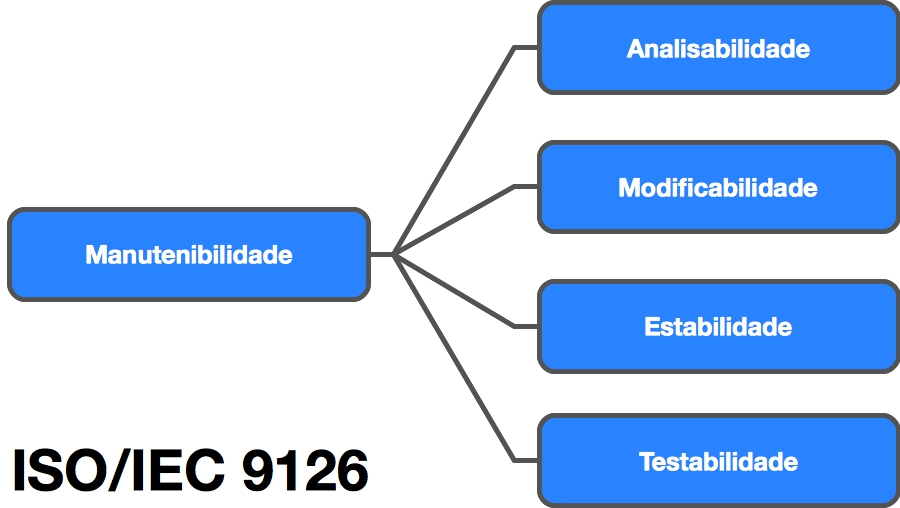
\includegraphics[width=0.5\textwidth]{imagens/subcaracteristica-manutenibilidade.jpg}
  \end{figure}
  
\end{frame}

\begin{frame}[t, fragile]{Índice de Manutenibilidade}
    \begin{block}{Definição:}
      \scriptsize{
      $MI = 171 - 5.2 \times \ln(aveV) - 0.23 \times aveV(g') 
        - 16.2 \times ln(aveLoc) + 50.0 \times \sin \sqrt{2.46 \times perCM}$
      }
    \end{block}
    \textbf{Onde:}
    \begin{tabular}{@{}>{$}l<{$}l@{}}
    aveV & average Halstead Volume\\
    aveV(g') & average extended cyclomatic complexity \\
    aveLoc & average count of lines of code (LOC)\\
    perCM & average percent of lines of comments
  \end{tabular}
       
\end{frame}

%\begin{frame}[allowframebreaks, t, fragile]{Sub-características da Manutenibilidade (ISO/IEC 9126)}
%        \begin{itemize}
%          \item \textbf{Analisabilidade}: medida de esforço necessário para diagnosticar deficiências ou causas de 
%            falhas, ou localizar as partes a serem modificadas para corrigir os problemas
%          \item \textbf{Modificabilidade}: medida de esforço necessário para realizar alterações, remover falhas ou 
%            para adequar o produto a eventuais mudanças de ambientes operacionais
%          \item \textbf{Estabilidade}: medida do risco de efeitos inesperados provenientes de modificações
%          \item \textbf{Testabilidade}: medida de esforço necessário para testar o software alterado
%        \end{itemize}
%
%\end{frame}

\begin{frame}[allowframebreaks, t, fragile]{Linhas de Produtos de Software}
    \begin{block}{Definição:}
        Um \alert{conjunto} de sistema de software que \alert{compartilham} intensivamente um \alert{conjunto comum} e gerenciado de funcionalidades \textcolor{Blue}{\cite{Clements2002}}. 
    \end{block}

    \begin{figure}[hbt]
      
      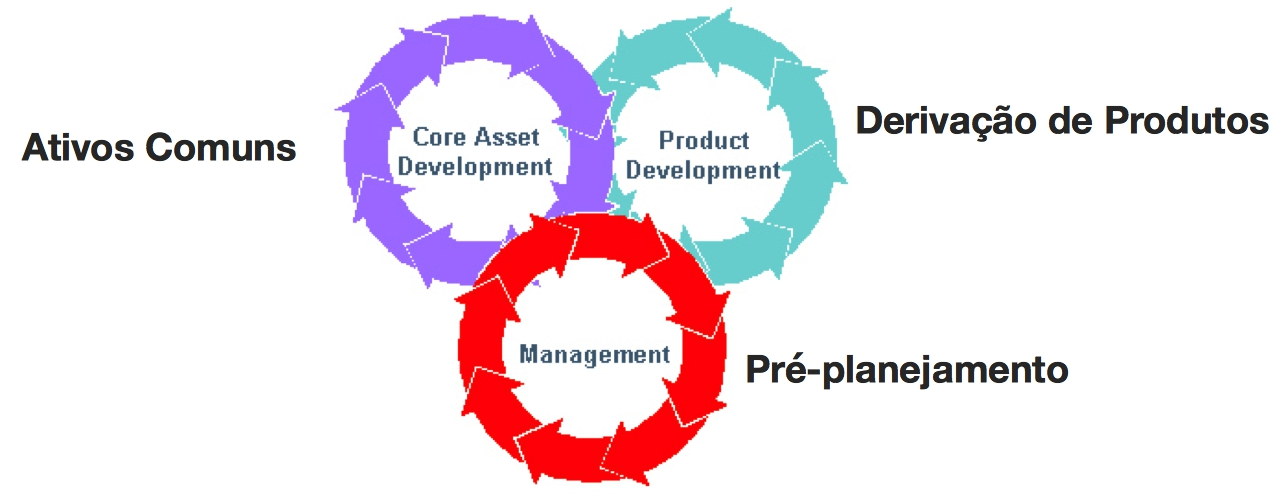
\includegraphics[width=0.8\textwidth]{imagens/atividades-essenciais-1}
      %\caption{Adaptada de \ref{Clements2001}.}
    \end{figure}
\end{frame}

\begin{frame}[allowframebreaks, t, fragile]{Feature Model}
    \begin{itemize}
     \item Feature model é um meio para \alert{representação} de um espaço de \alert{configuração} de todos os produtos de 
     uma \alert{família} de sistemas em termos de suas \textit{features}.
    \end{itemize}
    
    \begin{block}{Definição:}
      Features podem ser definidas como \alert{aspectos}, \alert{qualidades} ou \alert{características} de uma \alert{família} de sistemas.
    \end{block}
    
      \begin{figure}[hbt]
      
      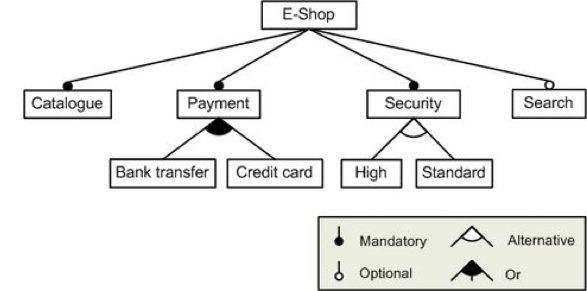
\includegraphics[width=0.8\textwidth]{imagens/exemplo-feature-model-1.jpg}
      %\caption{Adaptada de \ref{Clements2001}.}
    \end{figure}
\end{frame}

% \subsection{Importância}
% \begin{frame}[allowframebreaks, t, fragile]{Por que é Importante ?}
%    \begin{itemize}
%     \item Virtualmente quaisquer organização dependente de software tem vital interesse na redução das suas 
%       atividades de manutenção
%     
%     \item Manutenibilidade é amplamente aceita como um importante atributo de qualidade de sistemas de software
%       em razão do seu impacto econômico.
%       
%     \item Manutenibilidade de software tornou-se uma das mais importantes preocupações da indústria de software
%     \item F.Brooks reivindica "O custo total de manter um software é tipicamente 40 porcento ou mais do custo de desenvolvimento"
% 
%     \item Parik tem uma visão mais pessimista, reivindicando que de 45 a 60 é gasto com manutenção".
%     \item Corbi and Yourdon reivindica que a manutenibilidade de software e um dos maiores desafios para da década de 1990
%     
%    \end{itemize}
% \end{frame}
% 
% \subsection{Modelos de Avaliação da Manutenibilidade}
% \begin{frame}[allowframebreaks, t, fragile]{Modelos de Avaliação da Manutenibilidade}
%    \begin{itemize}
%     \item \textbf{Modelo de avaliação multidimensional}:   
%     \item \textbf{Modelo de regressão polinominal}: 
%     \begin{itemize}
%       \item Explora o relacionamento entre a manutenibilidade de software e as métricas de software. 
%     \end{itemize}   
%     \item \item \textbf{Medida de agregação de complexidade}:
%     \item \textbf{Análise de componentes principais}:
%     \item \textbf{Análise de fator}
%    \end{itemize}
% \end{frame}
% 
% \subsection{Manutenção versus Manutenibilidade}
% \begin{frame}[t, fragile]{Manutenção versus Manutenibilidade}
%     blabla
% \end{frame}

    \section{Desafios da Área de Estudo}
\begin{frame}[t, fragile]{Desafios Gerais}
    \begin{itemize}
      \item O estudo da manutenção de software é bastante \alert{desafiador} pois lida com fatores  técnicos e humanos.
%      \begin{itemize}
%	   \item técnicos: modularidade, acoplamento, o tamanho do código, sua complexidade e etc.
%	   \item humanos: estrutura de comunicação, familiaridade com o sistema, níveis de habilidade, liderança e etc. 
%      \end{itemize}
      
      
      %\item Yet most of the research studies have paid little attention to how software engineers understand the system and the information needed to perform a maintenance task. 
      \item Ao analisar a manutenibilidade deve-se observar três dimensões\cite{Hanafi2015}:
      \begin{itemize}
	     \item As \alert{pessoas} que executam manutenção de software.
	     \item Os \alert{objetivos} e as \alert{tarefas} da manutenção.
	     \item \underline{As \alert{propriedades} técnicas do sistema em consideração}
      \end{itemize}
      
    \end{itemize}
\end{frame}

\begin{frame}[t, fragile]{Desafios Específicos}
    \begin{itemize}
      \item A \alert{manutenção} em linhas de produtos é considerada mais \alert{complexa} do que em \alert{sistemas tradicionais} $\rightarrow$ \alert{modificações} em um módulo podem afetar \alert{diversos produtos}.
      \item A \alert{quantidade} de ferramentas e guidelines para auxiliar a manutenção ou aumentar a manutenibilidades da linhas são \alert{limitadas}  \cite {Vale2015}.
      
    \end{itemize}
\end{frame}
    \section{Artigos Estudados}
\begin{frame}[t, fragile]{Artigos}
    \begin{itemize}
      \item \textcolor{Green}{Artigo 1}: VALE, G. et al. Criteria and Guidelines to Improve Software Maintainability in Software Product Lines IEEE, abr. 2015. $\rightarrow$ \textbf{Básico}
      \item \textcolor{Blue}{Artigo 2}: BAGHERI, E.; GASEVIC, D. Assessing the maintainability of software product line feature models using structural metrics. Software Quality Journal, v. 19, n. 3, p. 579–612, set. 2011. $\rightarrow$ \textbf{Intermediário}
      \item \alert{Artigo 3}: CAFEO, B. et al. Towards Indicators os Instabilities in Software Product Lines: An Empirical Evaluation Metrics.  In Proceedings of the 35th International Conference on Software Engineering (ICSE). Piscataway, NJ: IEEE, 2013. $\rightarrow$ \textbf{Avançado}

    \end{itemize}
\end{frame}

    \subsection{Artigo 1}
\begin{frame}[t, fragile]{Artigo1: Ideias Básicas}
    \begin{itemize}
      \item \textcolor{Green}{Artigo 1}: VALE, G. et al. Criteria and Guidelines to Improve Software Maintainability in Software Product Lines IEEE, abr. 2015. $\rightarrow$ Básico
    \end{itemize}
\end{frame}

    
\begin{frame}[t, fragile]{Artigo 1: Objetivos}        
  \begin{figure}[hbt]
    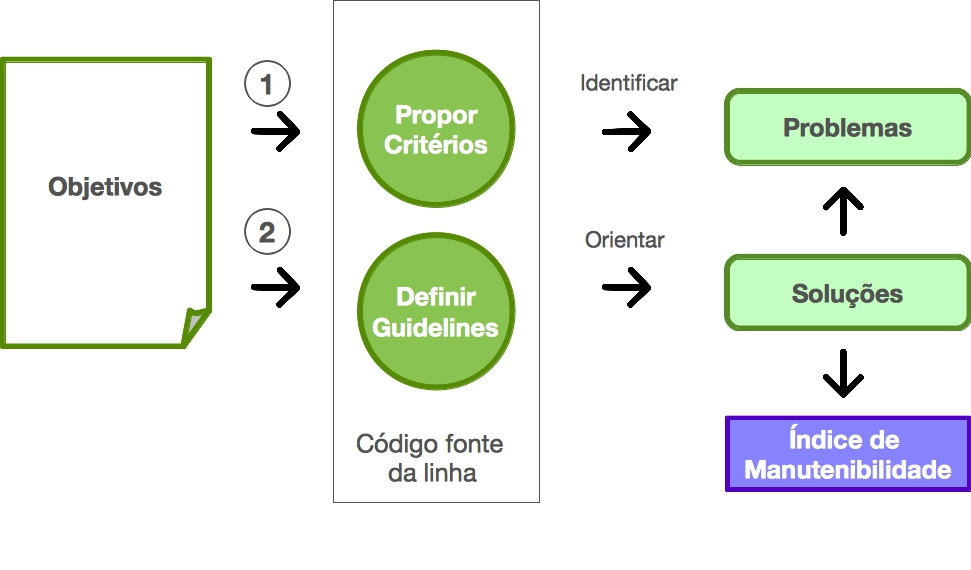
\includegraphics[scale=0.4]{imagens/artigo1-objetivos.jpg}
  \end{figure}
\end{frame}
    
\begin{frame}[allowframebreaks, t, fragile]{Artigo 1: Metodologia}
  \begin{enumerate}      
    \item Levantamento bibliográfico para escolha da linha, definição de critérios e \textit{guidelines}.
    \item Aplicações dos \textit{guidelines} separadamente e conjuntamente em \underline{seis produtos} da linha escolhida (TankWar).
    \item Cálculo do MI (antes e depois da aplicação dos \textit{guidelines}) e realização de análises estatísticas sobre os resultados
    
  \end{enumerate} 
\end{frame}
    
\begin{frame}[allowframebreaks, t, fragile]{Artigo 1: Resultados}
   \begin{figure}[hbt]
    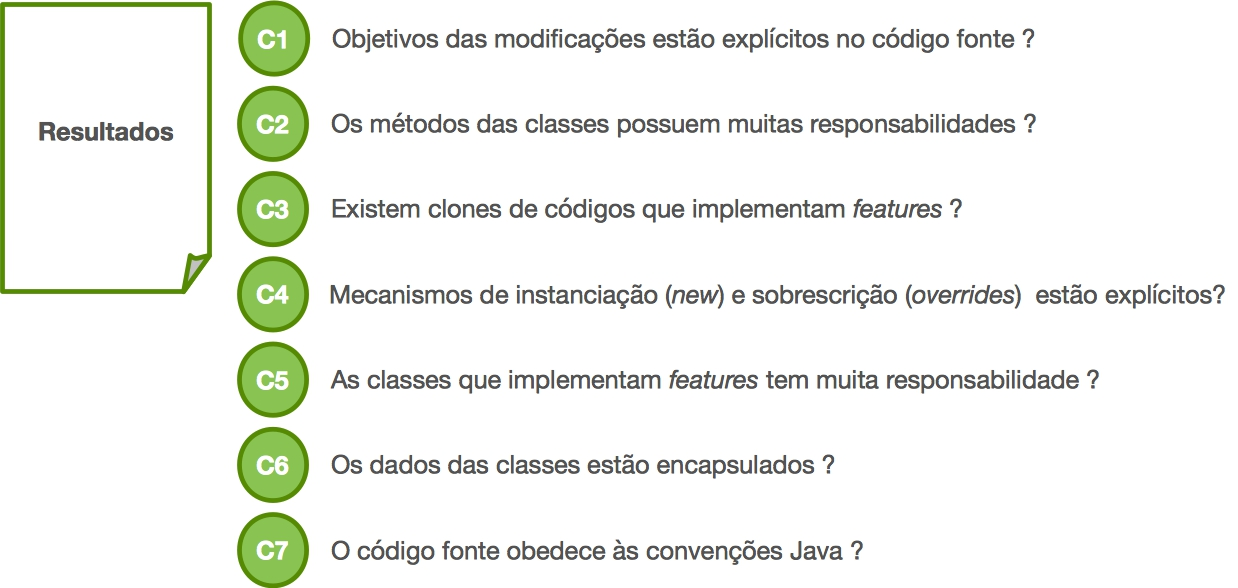
\includegraphics[scale=0.35]{imagens/artigo1-resultados-1.jpg}
  \end{figure}  
   \begin{figure}[hbt]
    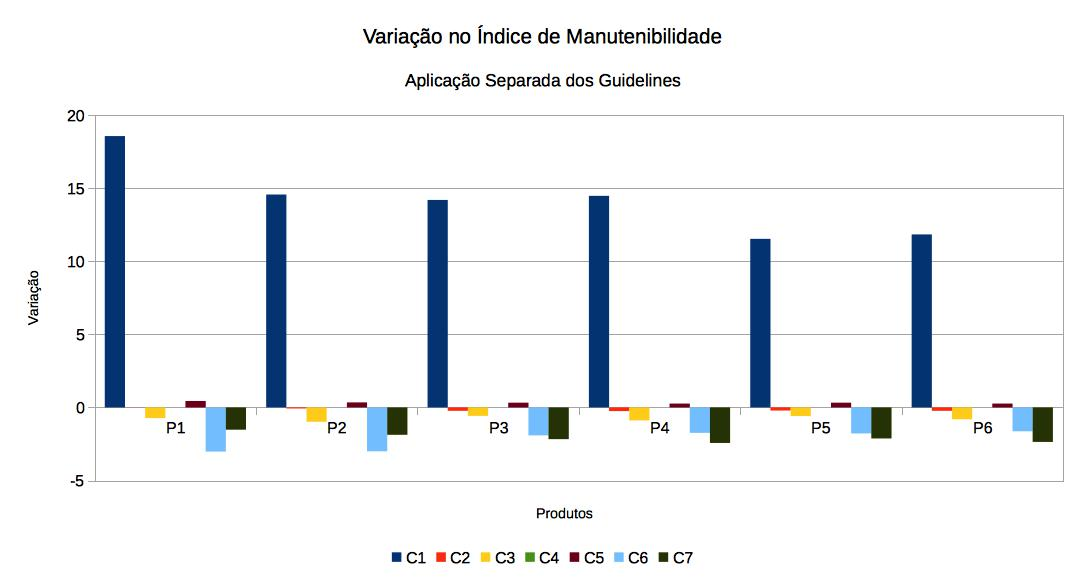
\includegraphics[scale=0.40]{imagens/artigo1-resultados-2.jpg}
  \end{figure} 
  \begin{figure}[hbt]
    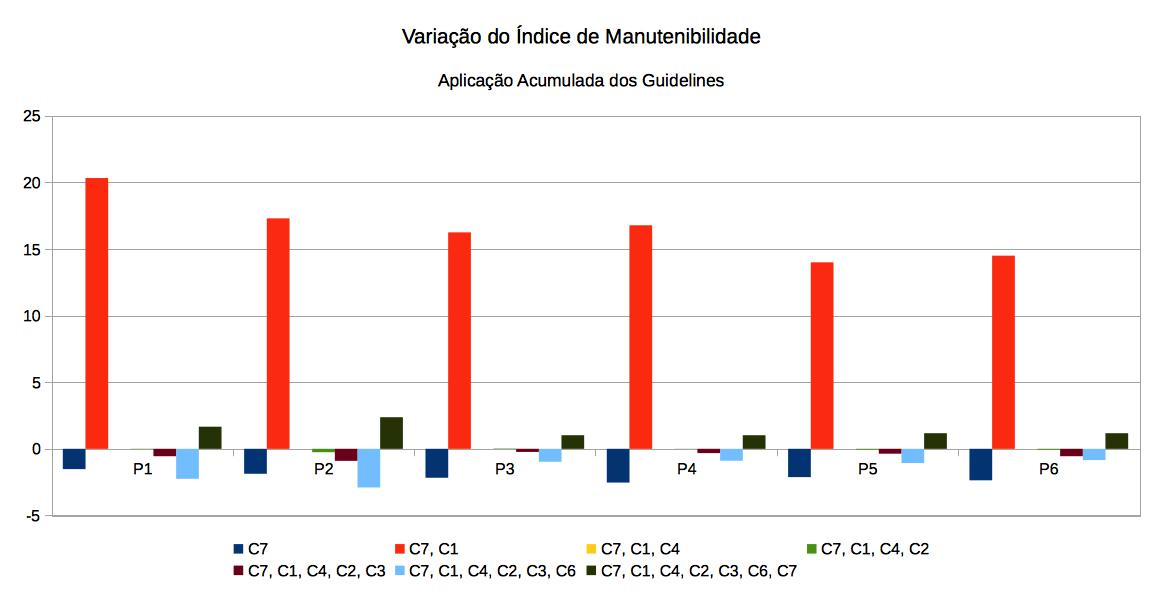
\includegraphics[scale=0.36]{imagens/artigo1-resultados-3.jpg}
  \end{figure} 
\end{frame}
    \subsection{Artigo 2}
\begin{frame}[t, fragile]{Artigo 2}
  \begin{itemize}
    \item \textcolor{Blue}{Artigo 2}: BAGHERI, E.; GASEVIC, D. Assessing the maintainability of software product line feature models using structural metrics. 
    Software Quality Journal, v. 19, n. 3, p. 579–612, set. 2011. 
  \end{itemize}
\end{frame}
    \begin{frame}[allowframebreaks, t, fragile]{Artigo 2: Objetivos}        
  \begin{figure}[hbt]
    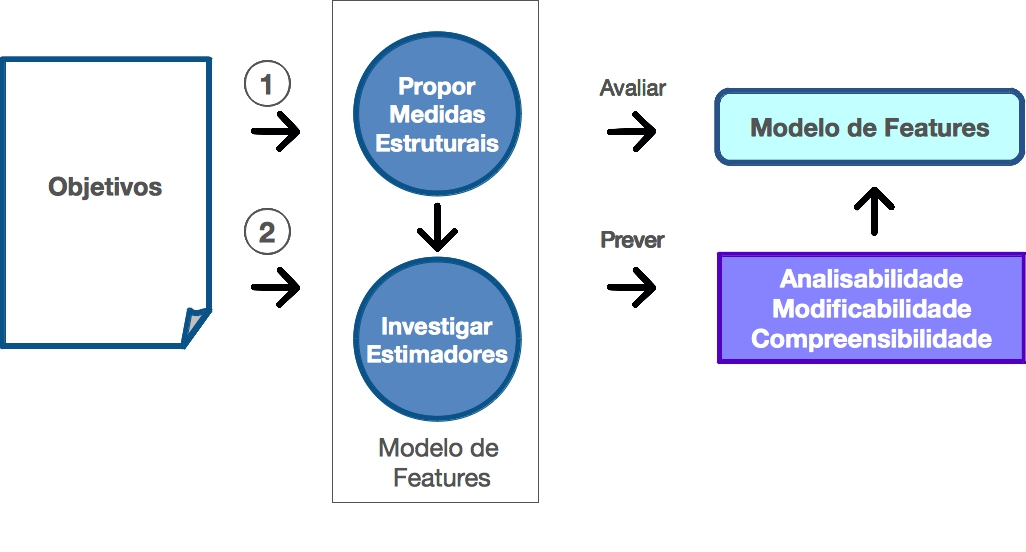
\includegraphics[scale=0.4]{imagens/artigo2-objetivos.jpg}
  \end{figure}
\end{frame}
    
\begin{frame}[t, fragile]{Artigo 2: Metodologia}
  \begin{enumerate}      
    \item Investigação de \alert{métricas estruturais} em modelos de \textit{features} e extração em \underline{quatorze linhas de produtos} registradas no SPLOT.
    \item Colhimento da \alert{percepção das sub-características} de manutenibiliade das linhas escolhidas através de questionários aplicados em um grupo de \underline{15 voluntários}.
    \item \alert{Correlação} das métricas extraídas com respostas dos questionários por meio de \alert{métodos estatísticos}.
  \end{enumerate} 
\end{frame}
    
\begin{frame}[t, fragile]{Artigo 2: Resultados}        
  \begin{figure}[hbt]
    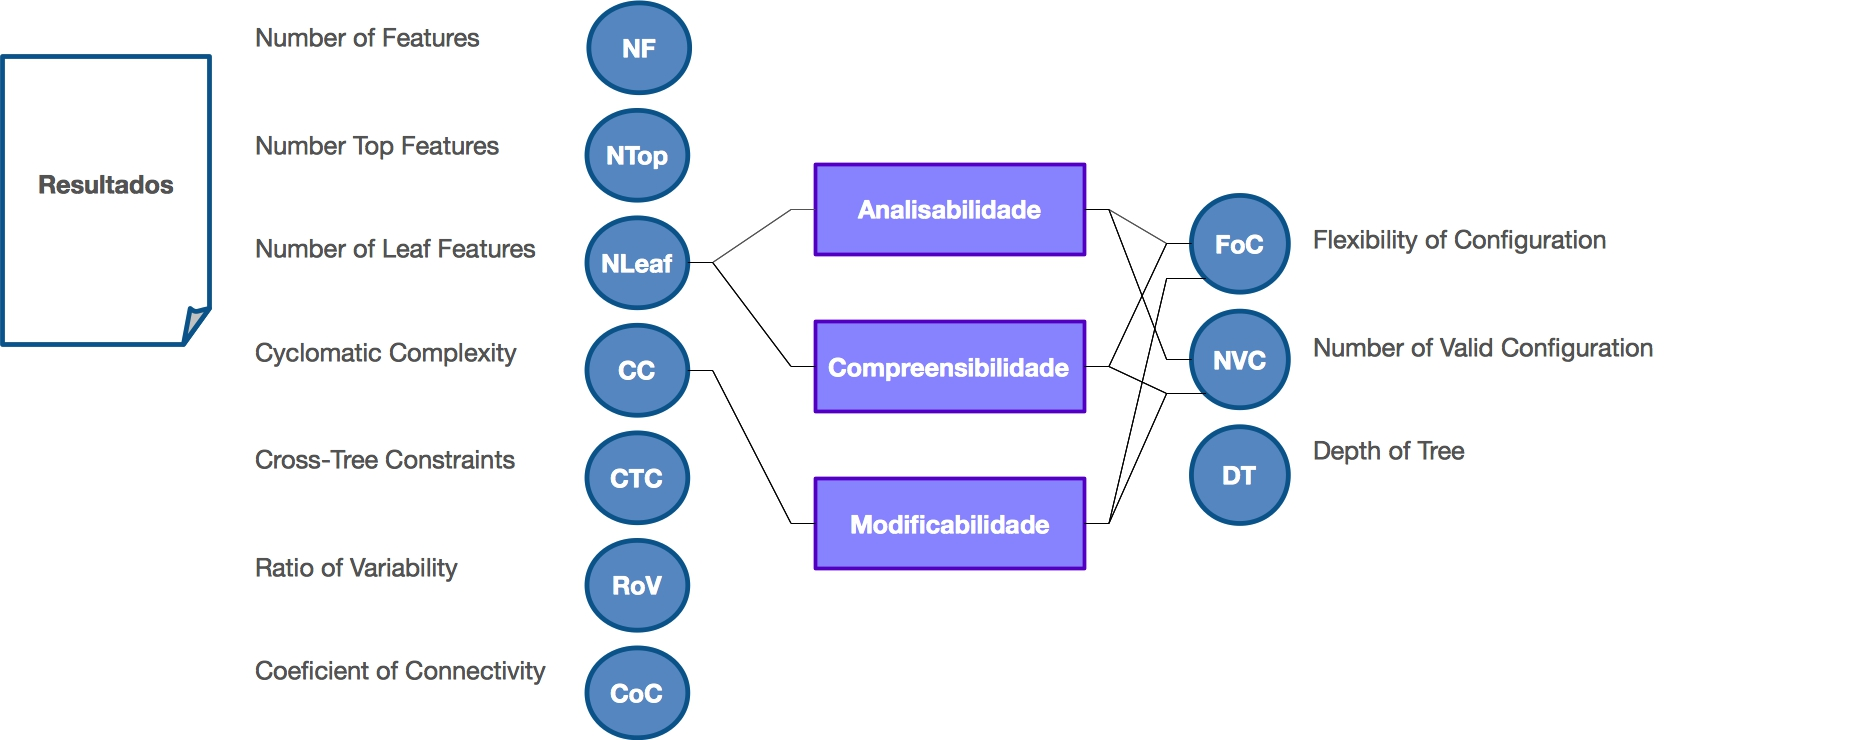
\includegraphics[scale=0.27]{imagens/artigo2-resultados-1.jpg}
  \end{figure}
\end{frame}
  

    \subsection{Artigo 3}
\begin{frame}[t, fragile]{Artigo 3}
  \begin{itemize}
         \item \alert{Artigo 3}: CAFEO, B. et al. Towards Indicators os Instabilities in Software Product Lines: A Empirical Evaluation Metrics.  In Proceedings of the 35th International Conference on Software Engineering (ICSE). Piscataway, NJ: IEEE, 2013.
  \end{itemize}
\end{frame}
    \begin{frame}[t, fragile]{Artigo 3: Objetivos}        
  \begin{figure}[hbt]
    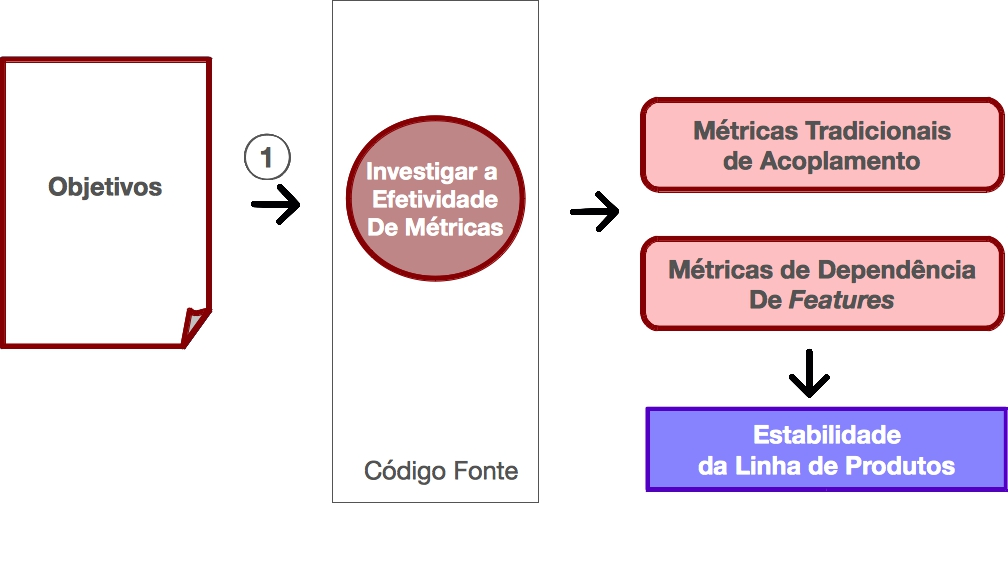
\includegraphics[scale=0.4]{imagens/artigo3-objetivos.jpg}
  \end{figure}
\end{frame}
    
\begin{frame}[allowframebreaks, t, fragile]{Artigo 3: Metodologia}
  \begin{enumerate}      
    \item \alert{Mapeamento} automatizado de \alert{elementos do código} para \alert{\textit{features}} em \underline{duas linhas de produtos} (GameUP e MobileMedia).
    \item Coleta de um conjunto de \alert{métricas} de acoplamento \alert{tradicionais} OO e AOP e de \alert{métricas} de dependência de \alert{\textit{features}}.
 
    \item Quantificação da \alert{instabilidades} através da medição de \alert{propagação de mudanças} em elementos  da linha de produto utilizando os \alert{dois} conjuntos de métricas.
  \end{enumerate} 
\end{frame}
    
\begin{frame}[allowframebreaks, t, fragile]{Artigo 3: Resultados}
  
          
  \begin{figure}[hbt]
    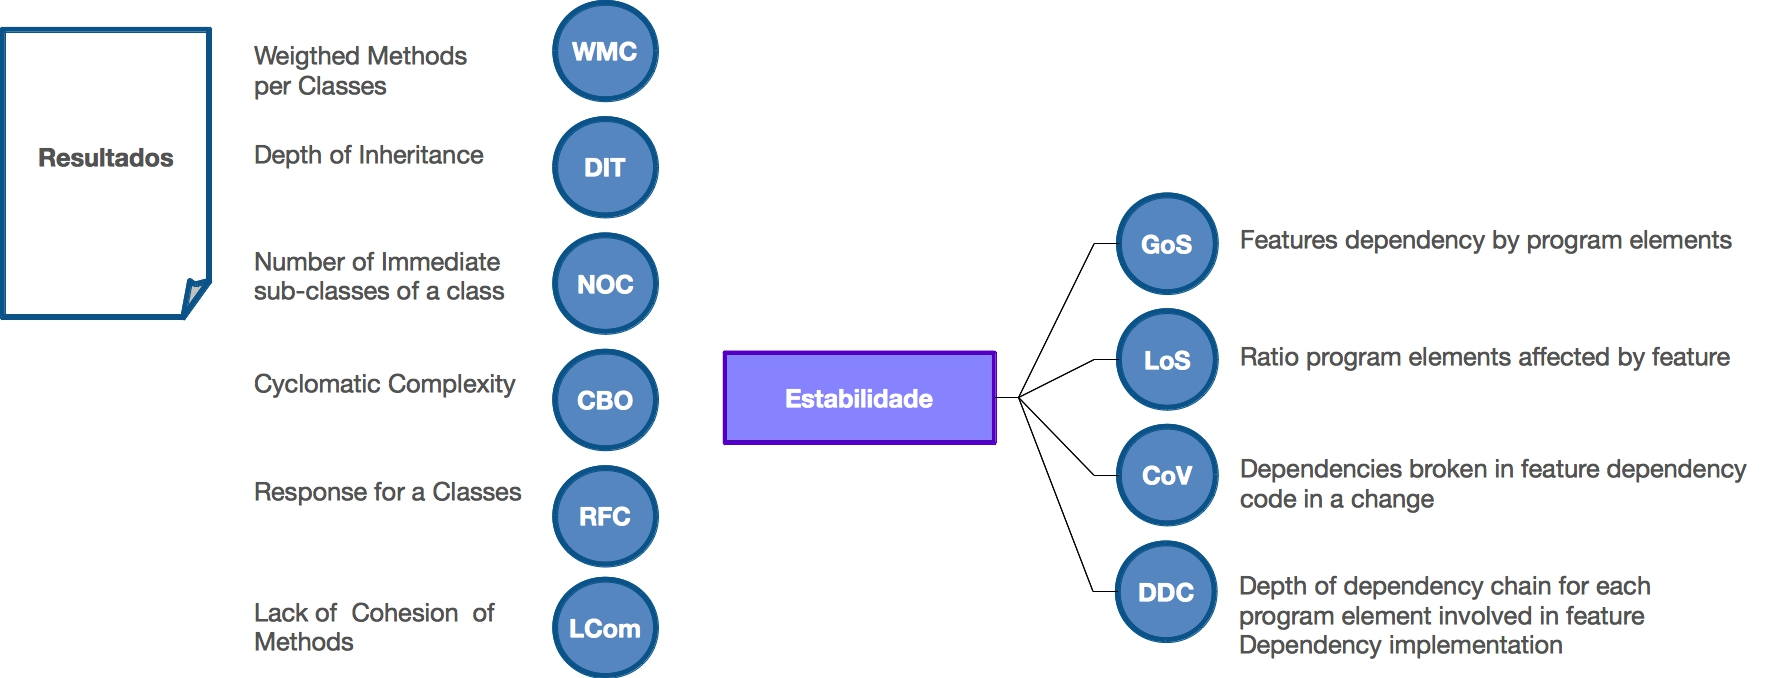
\includegraphics[scale=0.25]{imagens/artigo3-resultados-1.jpg}
  \end{figure}

%   \begin{table}\centering
%      \small
%      \begin{tabular}{@{} p{2cm}  p{8cm} @{}}
%	\toprule
%	  \textbf{Métrica} & \textbf{Descrição}      \\
%	  \midrule
%	  WMC   & Quantidade de operações por classe ou aspecto.\\
%	  DIT	& Profundidade da árvore de herança 	     \\
%	  NOC	& Quantidade de sub-classes ou sub-aspectos em um módulos \\
%	  CBO   & Acoplamento entre interfaces, classes e ou aspectos 	         \\
%	  RFC   & Quantidade de métodos ou advices executados em resposta a uma mensagem recebida.	 \\
%	  LCOM  & Quantidade de pares de operações trabalhando em campos diferentes de classes ou aspectos menos
%	   os pares de operações trabalhando com atributos em comum (Lack de coesão entre métodos)	 \\
%	  \bottomrule
%      \end{tabular}
%   \end{table}
%   
%   \framebreak
%   \begin{table}\centering
%      \small
%      \begin{tabular}{@{} p{2cm}  p{8cm} @{}}
%	\toprule
%	  \textbf{Métrica} & \textbf{Descrição}      \\
%	  \midrule
%    	GoS   & Quantidade de operações por classe ou aspecto.\\
%    	LoS	  & Profundidade da árvore de herança 	     \\
%    	CoV	  & Quantidade de sub-classes ou sub-aspectos em um módulos \\
%    	DDC   & Acoplamento entre interfaces, classes e ou aspectos\\
%	  \bottomrule
%      \end{tabular}
%   \end{table}

\end{frame}
    \section{Consolidação dos Resultados}
\begin{frame}[allowframebreaks, t, fragile]{Consolidação}
    \begin{itemize}
      \item Métricas apresentadas por artigo relacionadas à manutenibilidade de linhas de produtos.
    \end{itemize}
    \begin{table}\centering
      \small
      \begin{tabular}{@{} c r r r @{}}
      \toprule
      & \multicolumn{3}{c}{\textbf{Métricas}} \\
	  \textbf{Artigo} & \textbf{Apresentadas} & \textbf{Efetivas} & \textbf{\%}\\
	  \midrule
	   1 & 7 & 2 & 14\\
	  \midrule
	   2 & 10 & 5 & 50\\
	  \midrule
       3 & 10 & 4 & 40\\
	  \bottomrule
      \end{tabular}
   \end{table}  

%\framebreak
%    \begin{itemize}
%      \item Métricas apresentadas por artigo relacionadas às sub-características da Norma ISO-9126.
%    \end{itemize}
%    
%    \begin{table}\centering
%      \small
%      \begin{tabular}{@{} c p{1cm} p{1cm} p{1cm} p{1cm} @{}}
%      \toprule
%	  \textbf{Artigo} & \textbf{A} & \textbf{M} & \textbf{E}  & \textbf{T} \\
%	  \midrule
%	   1 & 0 & 0 & 0 & 7 \\
%	  \midrule
%	   2 & 0 & 7 & 0 & 0 \\
%	  \midrule
%       3 & 0 & 0 & 4 & 0 \\
%	  \bottomrule
%	  
%      \end{tabular}
%      
%      \tiny{(A)nalisabilidade, (M)odificabilidade, (E)stabilidade e (T)estabilidade 
%    \end{table}  
    
%\framebreak
%    \begin{itemize}
%      \item Métricas apresentadas por artigo relacionadas às atividades do Evolutionary Software Product Line Process\cite{Gomaa2005}.
%    \end{itemize}
%    
%    \begin{table}\centering
%      \captionsetup{singlelinecheck=off,labelfont=bf,labelsep=space}
%      \small
%      \begin{tabular}{@{} p{2cm} p{1cm} p{1cm} p{1cm} p{1cm}  p{1cm}@{}}
%      \toprule
%	  \textbf{Artigo} & \textbf{R} & \textbf{A} & \textbf{P} &\textbf{I} & \textbf{T} \\
%	  \midrule
%	   1 & 0 & 0 & 0 & 7 & 0 \\
%	  \midrule
%	   2 & 0 & 7 & 0 & 0 & 0\\
%	  \midrule
%       3 & 0 & 0 & 4 & 0 & 0\\
%	  \bottomrule
%	  
%      \end{tabular}
%      
%      \tiny{(R)equisitos, (A)nálise, (P)rojeto, (I)mplementação e  (T)estes}
%    \end{table}  
\end{frame}
    \section{Discussão dos Artigos}
\begin{frame}[t, fragile]{Discussão do Artigo 1}
    \begin{itemize}
 
      \item Os guidelines foram \alert{validados} em uma \alert{única} linha de produtos desenvolvida para fins acadêmicos
      
%       (Talvez isso torne mais críticos a contribuição negativa dos critérios apresentados) 
       \item O enunciado do critério C1 \alert{não está claro} no artigo. Ele não contemplaria o C7 ?       
      \item O enunciado dos critérios C2 e C5 não são \alert{objetivamente} verificáveis. 
%       \begin{itemize}
% 	\item o que se entende por "\underline{grande} ou \underline{muita} quantidade de responsabilidades de classes e métodos" ?.
%       \end{itemize}
       
      \item Os \textit{guidelines} de \alert{quatro} critérios \alert{reduziram} o MI da linha de produto estudada e para \alert{um} critério
	foi \alert{inócuo}. 
%       \begin{itemize}
% 	\item sugere-se a não adequação dessas orientações para linhas ou
% 	\item que MI deva ser ajustado para esse domínio.
%       \end{itemize}
      
     
      %Já que estudos apontam que a simples presença de linhas de comentários não contribuiem positivamente para a manutenibilidade.
    \end{itemize}
\end{frame}

\begin{frame}[t, fragile]{Discussão do Artigo 2}
    \begin{itemize}
     \item A utilização de critérios \alert{subjetivos} na coleta de dados é um ponto discutível.
     \item A compreensibilidade \alert{não está} definida na norma ISO/IEC 9126 como \alert{sugere} o artigo.
    \end{itemize}
\end{frame}

\begin{frame}[allowframebreaks, t, fragile]{Discussão do Artigo 3}
    \begin{itemize}
      \item Não apresenta as razões para a escolha das  \alert{duas linhas} (desenvolvidas com técnicas diferentes) para \alert{validação dos resultados}.
      \item O artigo utilizou o termo \alert{"instabilidade"} ao invés do \alert{"estabilidade"} como está na norma \alert{ISO/IEC 9126}.      
    \end{itemize}
\end{frame}
    \section{Produto Exemplo}
\begin{frame}[allowframebreaks, t, fragile]{Produto: Sistema de Gestão de Manutenção}
	\begin{columns}
	  	\begin{column}{0.45\textwidth}
	  		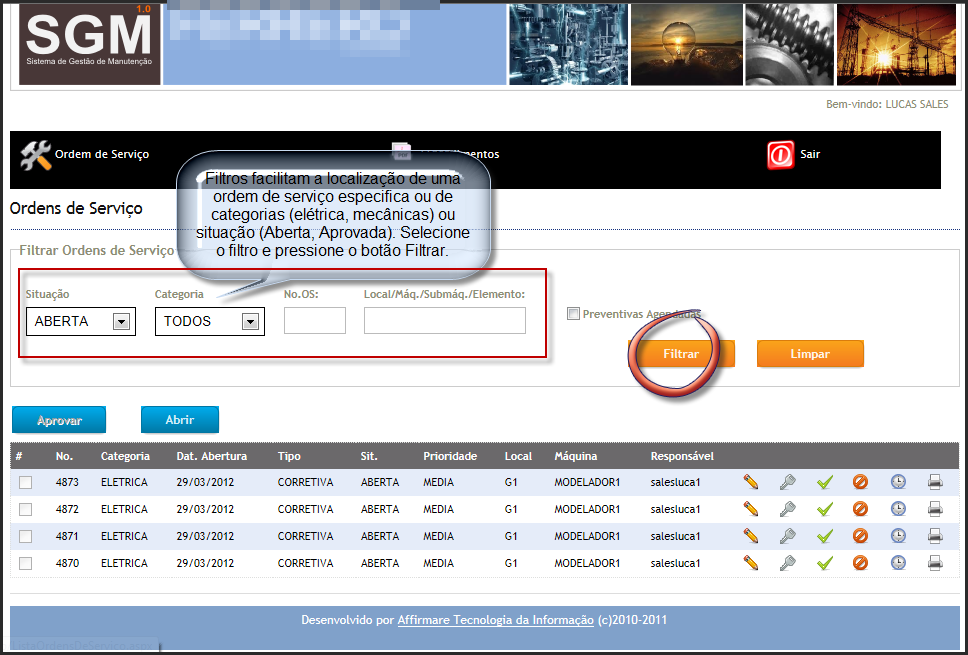
\includegraphics[width=1\textwidth]{imagens/sgm-01}
	  	\end{column}
	  	\begin{column}{0.45\textwidth}
	  		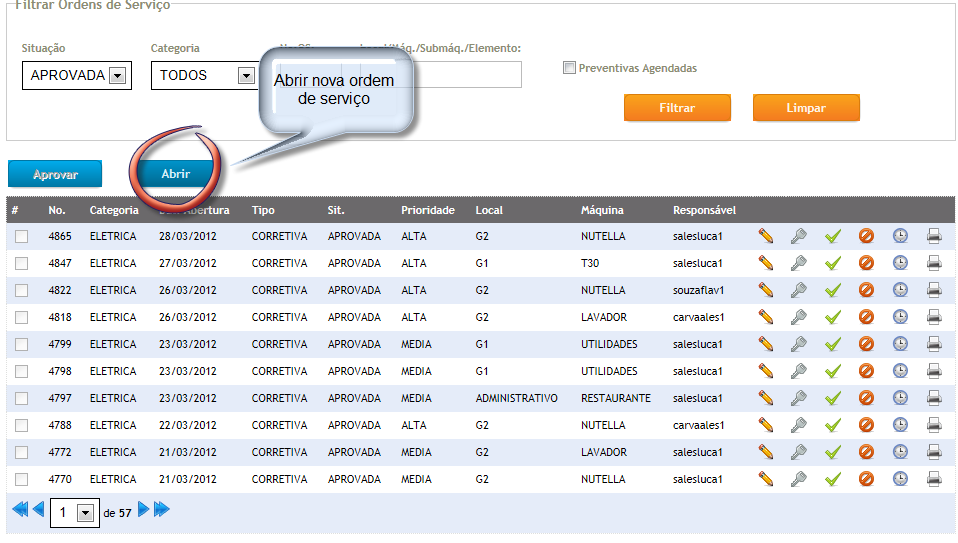
\includegraphics[width=1\textwidth]{imagens/sgm-02}
	  	\end{column}
	\end{columns}



	\framebreak
	
	\begin{columns}
		\begin{column}{0.45\textwidth}
			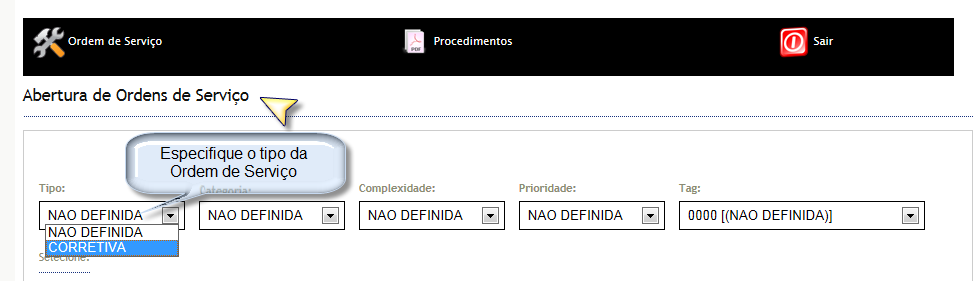
\includegraphics[width=1\textwidth]{imagens/sgm-03}
		\end{column}
		\begin{column}{0.45\textwidth}
			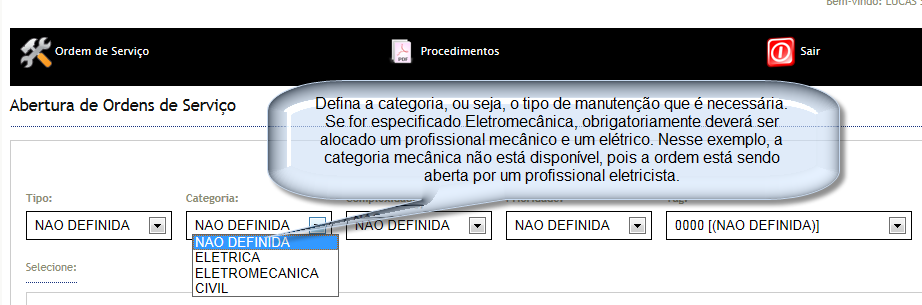
\includegraphics[width=1\textwidth]{imagens/sgm-04}
		\end{column}
	\end{columns}
	
	\framebreak
	
	\begin{columns}
		\begin{column}{0.45\textwidth}
			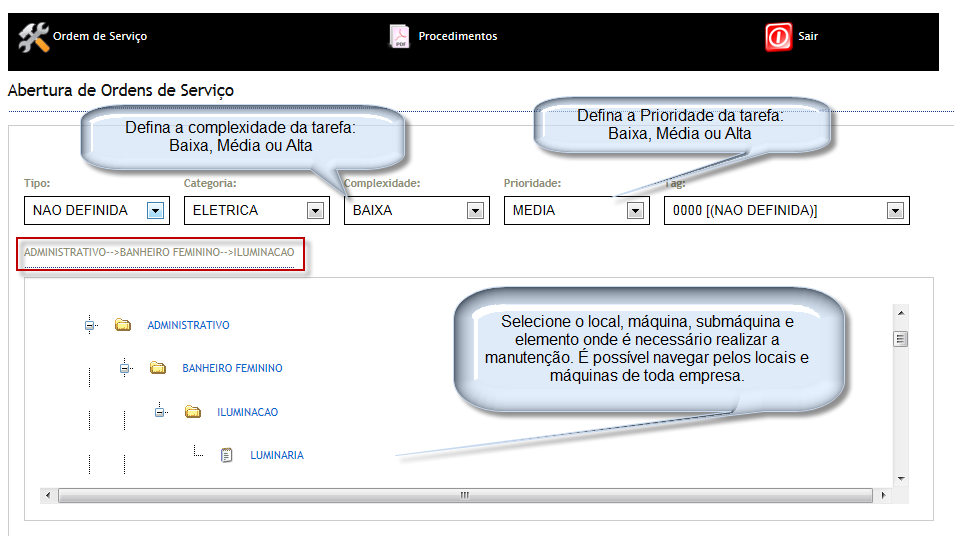
\includegraphics[width=1\textwidth]{imagens/sgm-05}
		\end{column}
		\begin{column}{0.45\textwidth}
			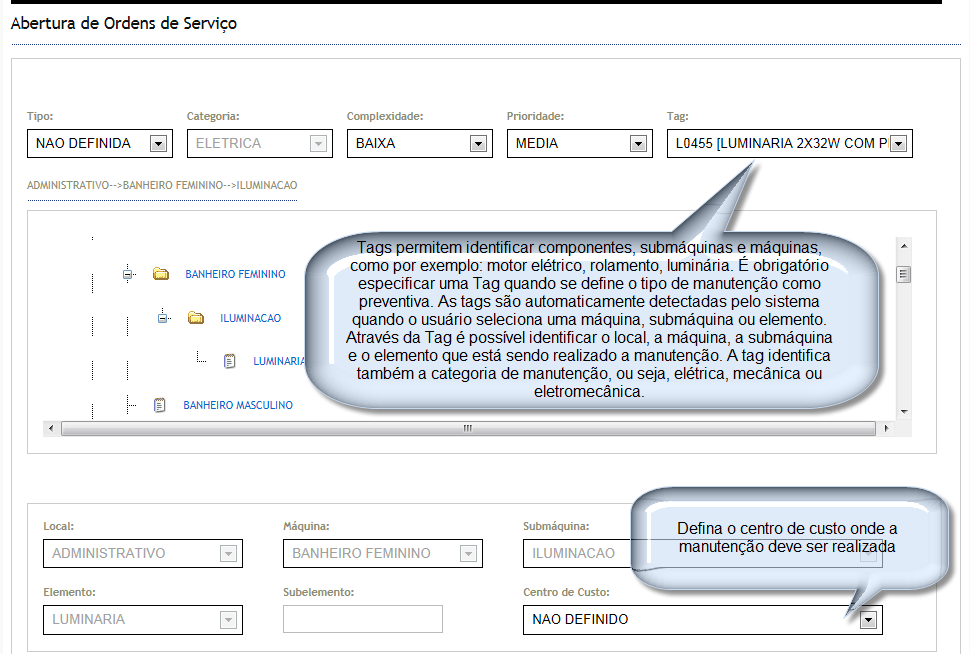
\includegraphics[width=1\textwidth]{imagens/sgm-06}
		\end{column}
	\end{columns}
	
	\framebreak
		
		\begin{columns}
			\begin{column}{0.45\textwidth}
				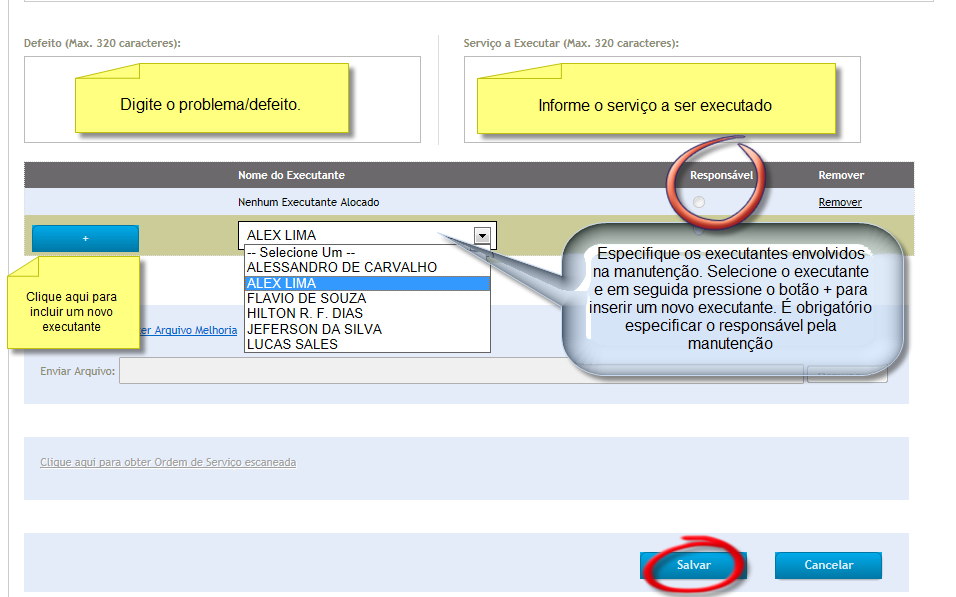
\includegraphics[width=1\textwidth]{imagens/sgm-07}
			\end{column}
			\begin{column}{0.45\textwidth}
				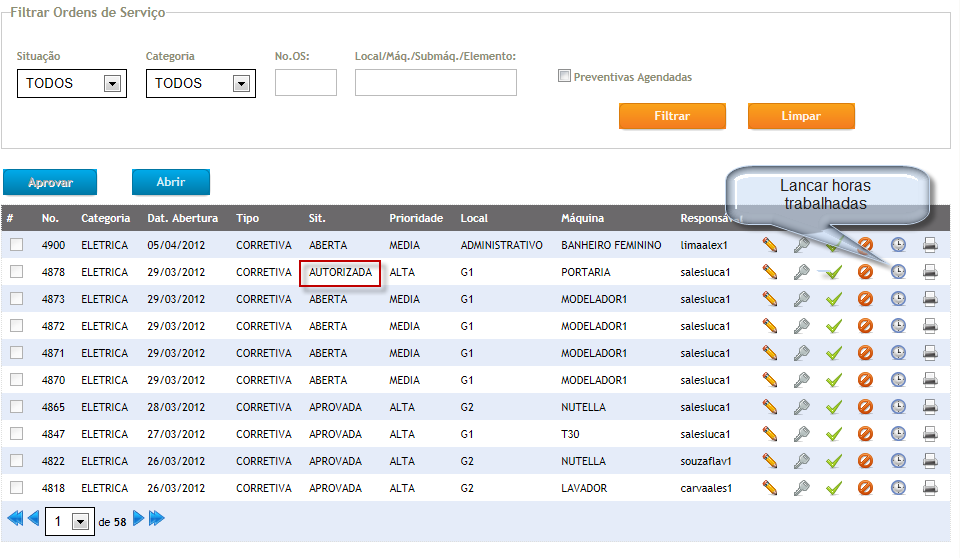
\includegraphics[width=1\textwidth]{imagens/sgm-08}
			\end{column}
		\end{columns}

	\framebreak
	
	\begin{columns}
		\begin{column}{0.45\textwidth}
			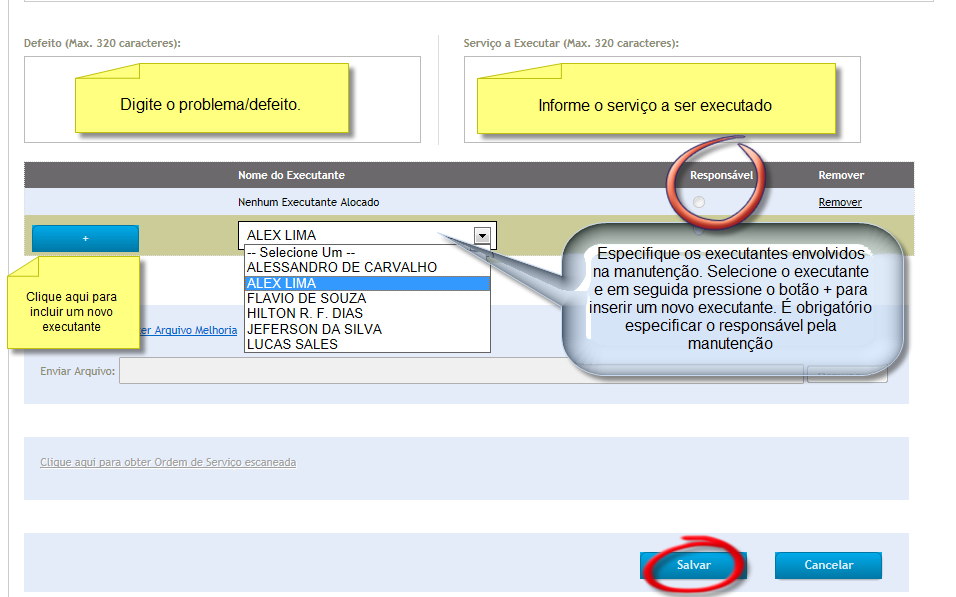
\includegraphics[width=1\textwidth]{imagens/sgm-07}
		\end{column}
		\begin{column}{0.45\textwidth}
			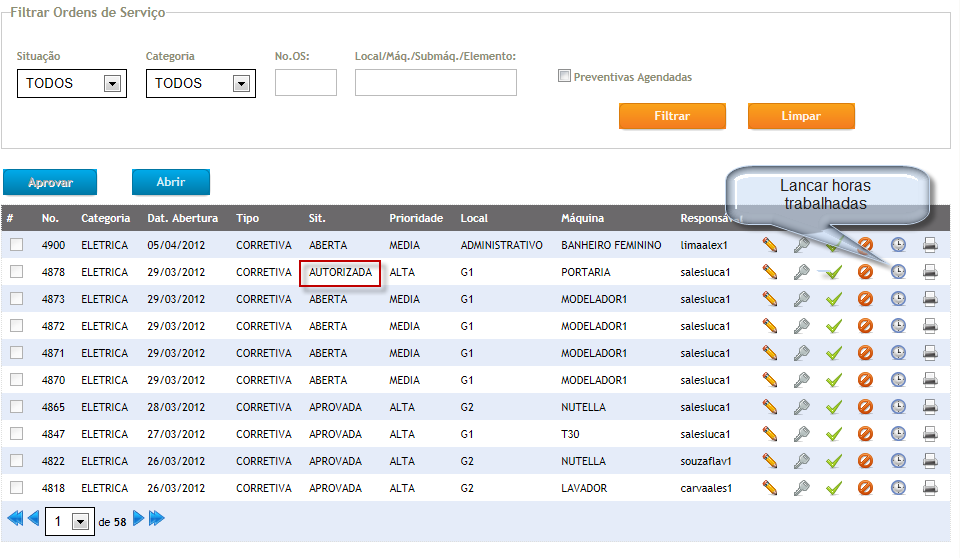
\includegraphics[width=1\textwidth]{imagens/sgm-08}
		\end{column}
	\end{columns}
	
\end{frame}
    \nocite{Bodker:2006}
\nocite{Bodker:2015}

    \section{Bibliografia}
\begin{frame}[t, fragile]{Bibliografia}
	\bibliography{Bibliografia}
\end{frame}

\end{document}

